
\section{Experiment and Results} 

\subsection{Implementation details} 

We used the same dataset used in CP-VTON, collected first for VITON. We used IoU and SSIM performance metrics for the same cloth retry-on cases for GMM and TOM. For final output quality measures, we used SSIM, Inception Score (IS)[9] and LPIPS[10] for different cloth try-on. The subjective qualities can be examined in Fig. 5/7.  Special comments are required for the IoU values, where CP-VTON (0.78) is slightly higher than CP-VTON+ (0.75). The un-expected results originated due to CP-VTON generating as in the current cloth shape. However, similar clothes are not always applicable, furthermore, it generates wrong shaped results for different clothes. Fig. 6 illustrates this with two typical example, plugging and normal tops

\subsection{Comparative Results}

\begin{figure}
\centering
%\includegraphics[height=6.5cm, scale=1]{figures/vton_result1.png} 
%\includegraphics[height=6.5cm, scale=1]{figures/vton_result2.png} 
\caption{VTON results}
\label{fig:vtonresults}
\end{figure}


Final, i.e., TOM results are evaluated with non-reference methods, LPIPS[10], IS[9] and SSIM. Our proposed method, CP-VTON+ outperforms CP-VTON in LPIPS with 0.1263 against 0.1397, in SSIM with 0.8076 over 0.7798, and in IS with 2.76 over 2.7417. The subjective evaluation shows significant visual improvements, especially in cloth textures such as logos and patterns (Fig. 7). We added the test results for all test cases for comparison between CP-VTON and CP-VTON+ in supplementary materials, together with the categorized comparison of SCM-based VTON, VITON and CP-VTON.


\subsection{Ablation Study}

Figure ~\ref{fig:ablation} we highlight the impact of the identified problems and improvement of the proposed method step-by-step through the ablation study of CP-VTON+. The first and second columns are target humans and try-on clothes, respectively. The third column is vanilla CVP-VTON results. The fourth column is when unchanged clothes and body parts are added to the reserved region inputs of TOM, retaining the original pants texture. The fifth column is when the mask loss function of TOM is updated with the target cloth area, making the texture and color of cloth sharp and vivid. Finally the sixth and last column is when the body masks are updated, replacing the skin area wrongly labelled as background and hair are removed from the reserved region input of GMM, making GMM can better cloth-and-hair-agnostic human representation.  


WHEN WE GET the GMM improvement, Where we can add this? may be the first step?

\begin{figure}
\centering
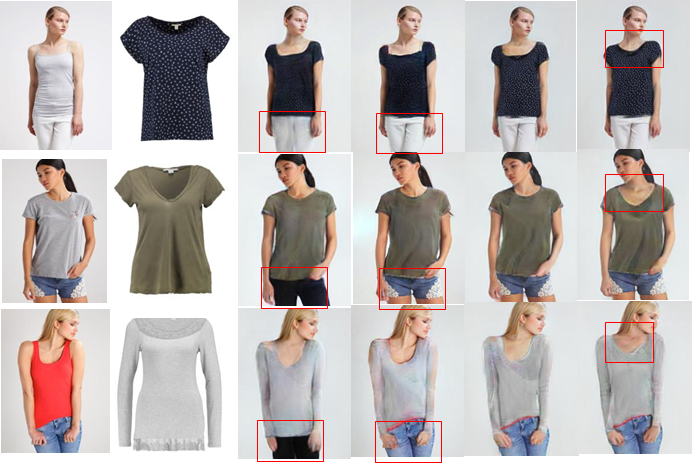
\includegraphics[height=6.5cm, scale=1]{figures/ablation.png} 
\caption{Ablation study of CP-VTON+. From left to right column. Target human, try-on cloth, CP-VTON, w. human representation, warped cloth mask and mask loss function updated, and CP-VTON+
}
\label{fig:ablation}
\end{figure}



\subsection{Known further issues}


Even though our modification  improve the VTON results a lot, and showing highly natural results, note that the dataset has limited samples for difficult cases, like the long sleeved, complicated shaped, or textured cloth and large posture target human. We amplify the key problems identified not try to list all the small problems. 

As Figure ~\ref{fig:gmmfailure} shows two typical failure cases due to the cloth warping. First row shows when the arms heavily covers the body area. The warped cloth does not match to the human body and TON failed in hiding the warping error. It is due to the limitation of STN (Spatial Transform Network). STN is originally developed for invert the (augmented) input images for different camera views and camera distortion. Non-rigid transforms, including TPS algorithms, cannot handle the strong 3D deformations of cloth.  Also the 3D poses induce self-occlusions. The TON network should recognized the cloth area and skin areas, like naked arms. One practical short-term solution would be to restrict the pose of target human image from the customer. And the long-term solution would be developed an 3D cloth deformation techniques for the GMM step, which is under studied by the authors. 

The second rows shows the another problems. Even without strong 3D posture of the target human, the warped cloth often shows un-realistic results. The accuracy for matching and warping of STN is not fully studied for VTON applications. 

%%%%%%%%
WE need to say something.
%%%%
    

The output image quality of all image-based VTON algorithms including ours depend upon the quality of input human representation, i.e., estimated joint locations and parsed human segmentation. The poses of target humans are usually (or forced) rather simple so that the state-of-the-art pose estimation algorithms can provide fairly accurate positions. However the quality of parsed human are not always good enough, especially when the target human wear complicated clothes. Also one can restrict the complexity of human images in pose and cloth style, but still the accuracy at the segmentation boundary sometimes affects the blended image results as shown in third row case in Fig ~\ref{fig:ablation}, where the pixels of the current top cloth, which is mislabelled as bottom cloth, remained in the blending result. There fore high quality human parsing algorithm especially around boundaries are required.   


\begin{figure}
\centering
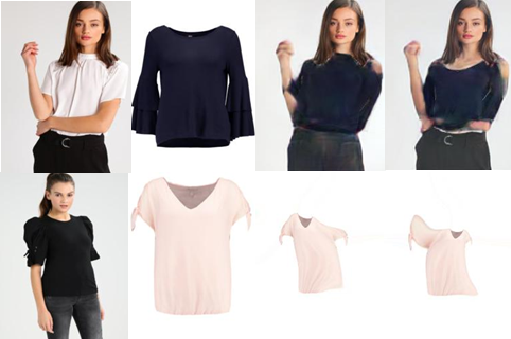
\includegraphics[height=6.5cm, scale=1]{figures/gmmfailure.png} 
\caption{Cloth Warping Failure of CP-VTON+. From left to right column. Target human, try-on cloth, CP-VTON, and CP-VTON+  (Why not same first and second ??)
}
\label{fig:gmmfailure}
\end{figure}
 